\documentclass[11pt,aspectratio=169,xcolor=dvipsnames]{beamer}
\usepackage[utf8]{inputenc}
\usepackage[T1]{fontenc}
%check out: https://www.matthiaspospiech.de/latex/templates/beamer/preambel/beamer-fonts/
%\usepackage{cmbright} 


\usepackage{tikz}
\usetikzlibrary{cd}
\usetikzlibrary{shapes.geometric,positioning,decorations.pathmorphing,}
\usetikzlibrary{mindmap}
\usetikzlibrary{shapes.multipart}
%for pyramid: https://tex.stackexchange.com/questions/110522/how-to-elegantly-create-a-pyramid-hierarchy-in-tikz
\usetikzlibrary{decorations.pathreplacing}
%For diagrams
%For arrows
\usepackage{marvosym}
\usepackage{amsmath,amssymb,amsthm}
\usepackage{stmaryrd}
\usepackage{bbm}

\renewcommand{\div}{\operatorname{div}}
\newcommand{\curl}{\operatorname{curl}}
\newcommand{\diffb}{\partial_{\bm{b}}}
\newcommand{\wh}{ \ \vert \ }
\renewcommand{\O}{\mathcal{O}}
\newcommand{\sth}{\sum_{T \in \mathcal{T}_h}}
\newcommand{\stn}{\sum_{\tau \in \mathcal{T}_n}}
\newcommand{\sfh}{\sum_{F \in \mathcal{F}_h}}
\newcommand{\sfn}{\sum_{F \in \mathcal{F}_n}}
\newcommand{\Th}{\mathcal{T}_h}
\newcommand{\Fh}{\mathcal{F}_h}
\newcommand{\Tn}{\mathcal{T}_n}
\newcommand{\Fn}{\mathcal{F}_n}
%Spaces
\newcommand{\N}{\mathbb{N}}
\newcommand{\X}{\mathbb{X}}
\newcommand{\Xn}{\X_n}
\newcommand{\XT}{\X_{\Tn}}
\newcommand{\XF}{\X_{\Fn}}
\newcommand{\Y}{\bm{Y}}
\newcommand{\V}{\bm{V}}
\newcommand{\W}{\bm{W}}
\newcommand{\Z}{\bm{Z}}
\newcommand{\G}{\bm{G}}
\newcommand{\bR}{\bm{R}}
\newcommand{\D}{\bm{D}}
\newcommand{\bPc}{\bm{\mathcal{P}}}

\DeclareMathOperator{\hess}{Hess}

\newcommand{\seq}[1]{(#1_n)_{n \in \N}}
\newcommand{\dgjump}[1]{ \llbracket #1 \rrbracket}
\newcommand{\dgavg}[1]{ \{\!\!\{#1\}\!\!\} }
\newcommand{\hdgjump}[1]{ \llbracket \underline{#1} \rrbracket}
\newcommand{\Pconv}{\overset{\scriptscriptstyle P}{\rightarrow}}
\newcommand{\Qconv}{\overset{\scriptscriptstyle Q}{\rightarrow}}
\newcommand{\PQconv}{\overset{\scriptscriptstyle PQ}{\rightarrow}}
\DeclareMathOperator{\coker}{coker}
\DeclareMathOperator{\ran}{ran}
\DeclareMathOperator{\nsp}{ker}
\DeclareMathOperator{\codim}{codim}
\DeclareMathOperator{\ind}{ind}
\DeclareMathOperator{\Hess}{Hess}
\DeclareMathOperator{\nran}{numran}
\DeclareMathOperator{\supp}{supp}
\newcommand{\ddiv}{\div_{\nv}^n}
\newcommand{\ddiffb}{\D^n_{\boldb}}

\newcommand{\dom}{\mathcal{O}}

\newcommand{\opd}{(\omega+i\diffb+i\Omega\times)}
\newcommand{\dopd}{(\omega+i\ddiffb+i\Omega\times)}

%Bold symbols
%Lower case
\newcommand{\nv}{\bm{\nu}}
\newcommand{\bpsi}{\bm{\psi}}
\newcommand{\bxi}{\bm{\xi}}
\newcommand{\boldu}{\bm{u}}
\newcommand{\boldv}{\bm{v}}
\newcommand{\boldw}{\bm{w}}
\newcommand{\boldz}{\bm{z}}
\newcommand{\boldx}{\bm{x}}
\newcommand{\boldf}{\bm{f}}
\newcommand{\boldg}{\bm{g}}
\newcommand{\boldq}{\bm{q}}
\newcommand{\boldb}{\bm{b}}
\newcommand{\boldr}{\bm{r}}
%Upper case
\newcommand{\bL}{\bm{L}}
\newcommand{\boldL}{\bm{L}}
\newcommand{\boldH}{\bm{H}}
\newcommand{\boldC}{\bm{C}}
\newcommand{\boldQ}{\bm{Q}}
\newcommand{\boldW}{\bm{W}}


\newcommand{\spl}{\langle}
\newcommand{\spr}{\rangle}

\newcommand{\topdecomp}{\oplus^{\mathcal{T}}}

\newcommand{\smzero}{\setminus \{0\}}

\newcommand{\lami}{\lambda^{(i)}}
\newcommand{\ei}{e^{(i)}}
\newcommand{\ui}{u^{(i)}}

%Solution operators
\newcommand{\AnDG}{A_n^{\text{DG}}}

%m matrix
\newcommand{\mat}{\underline{\underline{m}}}

%Facet h
\newcommand{\h}{\mathfrak{h}}
\newcommand{\Id}{\operatorname{Id}}
\newcommand{\tr}{\operatorname{tr}}
\newcommand{\Gjump}{\Gamma_{\dgjump{\cdot}_{\nv}}}
\newcommand{\Ijump}{\mathcal{I}_{\dgjump{\cdot}_{\nv}}}
\newcommand{\jnorm}[1]{\Vert #1 \Vert_{\Fn,1/2}}
\newcommand{\wjnorm}[1]{\Vert #1 \Vert_{\Fn,1/2,c_s^2 \rho}}

\newcommand{\matii}{\underline{\underline{m_2}}}

\usepackage{pgfplots,pgfplotstable}
\usepgfplotslibrary{colorbrewer,groupplots}
\usepackage{caption}
\pgfplotsset{compat=1.18}


%from: https://tex.stackexchange.com/questions/381591/using-tikzfillbetween-to-color-between-two-curves
\usetikzlibrary{intersections, pgfplots.fillbetween}

%find colors at https://colorbrewer2.org/#type=qualitative&scheme=Set1&n=5
\pgfplotsset{
% initialize Set1-5:
cycle list/Set1-5,
% combine it with ’mark list*’:
cycle multiindex* list={
mark list*\nextlist
Set1-5\nextlist
},
}

\pgfplotsset{
    discard if not/.style 2 args={
        x filter/.append code={
            \edef\tempa{\thisrow{#1}}
            \edef\tempb{#2}
            \ifx\tempa\tempb
            \else
                \def\pgfmathresult{inf}
            \fi
        }
    }
}



\usepackage{bm}

%\newcommand{\boldu}{\bm{u}}
%\newcommand{\nv}{\bm{\nu}}
%\newcommand{\bL}{\bm{L}}

%\newcommand{\dom}{\mathcal{O}}

%For comment environment
\usepackage{verbatim}
%for icons
\usepackage{fontawesome}

\usepackage{caption}
\usepackage{subcaption}

\usepackage{adjustbox}


\usepackage{XCharter}
%\usefonttheme{professionalfonts}

\input{pgfplt.tex}

\usepackage{pgfplots,pgfplotstable}
\usepgfplotslibrary{colorbrewer,groupplots}

%for checklist: https://tex.stackexchange.com/questions/321048/checklist-in-beamer-using-enumitem-package
\usepackage{pifont}


%flowchart: https://texample.net/tikz/examples/simple-flow-chart/
\usetikzlibrary{shapes,arrows}
\tikzstyle{block} = [rectangle, draw, fill=white!20, 
    text width=10em, text centered, rounded corners, minimum height=2em]
\tikzstyle{line} = [draw, -latex']


\usetheme{Slim}

\definecolor{GOE}{RGB}{35,95,150}
\definecolor{sfb}{HTML}{0070c0}
\definecolor{CRCLB}{RGB}{150,195,235}

\newcommand{\nicearrow}[2]{\raisebox{#2}{\resizebox{0.45cm}{!}{\color{#1}{\MVRightArrow}\color{black}}}}


% \highlight[<colour>]{<stuff>}
\newcommand{\highlight}[2][yellow]{\mathchoice%
  {\colorbox{#1}{$\displaystyle#2$}}%
  {\colorbox{#1}{$\textstyle#2$}}%
  {\colorbox{#1}{$\scriptstyle#2$}}%
  {\colorbox{#1}{$\scriptscriptstyle#2$}}}%


\DeclareFontFamily{OT1}{pzc}{}
\DeclareFontShape{OT1}{pzc}{m}{it}{<-> s * [1.10] pzcmi7t}{}
\DeclareMathAlphabet{\mathpzc}{OT1}{pzc}{m}{it}
\newcommand{\DtN}{\mathpzc{DtN}}
\newcommand{\dtn}{\mathpzc{dtn}}

\begin{document}

\begin{frame}[plain]{}
  % Background image
  \begin{tikzpicture}[remember picture,overlay]
    \thispagestyle{empty}
    \node
    [ 
        scale=1.1,
        fill=white,    
        below =0.5cm,
        align=right,
        minimum height=0.08\textwidth,
        minimum width=0.75\textwidth,
        text width=0.9\textwidth,   
     ] (ucllogo) at (current page.north)
     {
     %\includegraphics[height=0.9cm,keepaspectratio]{crc_logo.png}\\
     };  
    \node
    [ 
        scale=1.1,
        %fill=white,    
        below =0.5cm,
        align=left,
        minimum height=0.08\textwidth,
        minimum width=0.75\textwidth,
        text width=0.9\textwidth,   
     ] (logo) at (current page.north)
     {
     \includegraphics[height=0.9cm,keepaspectratio]{GOE_logo.png}\\
     };  
    \node
    [
        scale=1.2,
        fill=white,    
        below =0.7cm of logo,
        align=center,
        minimum height=0.08\textwidth,
        minimum width=0.75\textwidth,
        text width=0.9\textwidth,       
    ](title)
    {
      \color{white}   
         \LARGE \bfseries \color{black}{Analysis and approximation of the nematic Helmholtz--Korteweg equation}
    };
    \node
    [
        align=center,
        %fill=sfb!20,
  %       %rounded corners,
  %       inner xsep=15pt,
  %       inner ysep=10pt, 
        minimum width=\textwidth,
        text width=\textwidth, 
        below of = title,
        anchor = title.south,
        below = 0.4cm
     ] (author)
    {\large
    \textcolor{black}{Patrick E. Farrell$^1$, \underline{Tim van Beeck}$^2$, Umberto Zerbinati$^1$}
    };

    \node
    [ 
      align=center,
      fill=none, %blue!50!black!40,
         below=0.4cm of author, % and -3cm of author,
         anchor = north,
         minimum height=0.1\textheight,
         minimum width=0.46\textwidth,
         text width=0.8\textwidth,
     ] (date)
     {\phantom{a}$^1$University of Oxford; 
      \phantom{a}$^2$University of Göttingen\\
     };

     \node
    [ 
      align=center,
      fill=none, %blue!50!black!40,
         below=2cm of author, % and -3cm of author,
         anchor = north,
         minimum height=0.1\textheight,
         minimum width=0.46\textwidth,
         text width=0.95\textwidth,
     ] (conference)
     {
      Applied Mathematics Seminar, Pavia, Dec. 10th, 2024
     };
\end{tikzpicture}
\end{frame} 
\addtocounter{framenumber}{-1} 


\begin{frame}{Introduction}
  \begin{minipage}{0.7\textwidth}
    \begin{itemize}
      \item \alert{Goal:} describe time-harmonic acoustic wave propagation in a \alert{nematic liquid crystal} 
      \item<2-> Korteweg-fluid: $\underline{\underline{\sigma}} = p \underline{\underline{I}} - u_1 \rho (\nabla \rho \otimes \nabla \rho)$
      \item<3-> nematic LC can be considered as a Korteweg-fluid:
      \begin{equation*}
        \underline{\underline{\sigma}} = p \underline{\underline{I}} - u_1 \rho (\nabla \rho \otimes \nabla \rho) - u_2 (\nabla \rho \cdot \bm{n}) \nabla \rho \otimes \bm{n}
      \end{equation*}
      \item<4->[\nicearrow{GOE}{-0.07cm}] time harmonic acoustic waves described by the \alert{nematic Helmholtz--Korteweg} equations! 
      \item<4->[\nicearrow{GOE}{-0.07cm}] how does the alignment of the nematic field influence the propagation of the acoustic wave? 
    \end{itemize}
  \end{minipage}
  \hfill
  \begin{minipage}{0.29\textwidth}
    \begin{center}
      \begin{tikzpicture}
        \node at (0,0) {\includegraphics[width=2cm,keepaspectratio]{ActaNLC.png}};
        \node[align=center,font=\tiny\linespread{0.95}\selectfont] at (0,-2.5) {\tiny \color{gray} W. Wang, L. Zhang, P. Zhang, \\ \tiny \color{gray} \emph{Modelling and computation of liquid crystals.} \\ \tiny \color{gray} Acta Numerica, 2021.};
      \end{tikzpicture}
    \end{center}
  \end{minipage}
\end{frame}


\begin{frame}{Nematic Helmholtz--Korteweg equation\footnotemark}
  Given $f \in L^2(\Omega)$, find $u : \Omega \to \mathbb{C}$ s.t. 
  \begin{alignat*}{2}
    \alpha \Delta^2 u + \beta \nabla \cdot \nabla(\bm{n}^T (\mathcal{H} u) \bm{n}) - \Delta u - k^2 u &= f \quad &&\text{in } \Omega, \\
    \mathcal{B}u &= (0,0) \quad &&\text{on } \partial \Omega.
  \end{alignat*}
  \begin{itemize}
    \item $\Omega \subset \mathbb{R}^d$, $d = 2,3$, bounded Lipschitz domain;
    \item $\alpha, \beta:$ constitution parameters;
    \item $\mathcal{H}$: Hessian;
    \item $\bm{n}$: orientation of the nematic field ($\Vert \bm{n} \Vert = 1$);
    \item $k = \omega / c$: (classic) wave-number;
    \item $\mathcal{B}$: encodes the boundary conditions;
  \end{itemize}
  \footnotetext[1]{\tiny P.E. Farrell, U. Zerbinati, \emph{Time-harmonic waves in Korteweg and nematic-Korteweg fluids.} arXiv, 2024.}
  \begin{center}
    \begin{tikzpicture}[overlay]
      \draw (4,1.5) rectangle (6,3.5);
      \node at (5.5,3) {\footnotesize $\Omega$}; 
      \node at (5,3.7) {\footnotesize $\mathcal{B}$};
      \draw[-stealth,line width=1.5pt] (4.25,1.75) -- (5.75,1.75);
      \draw[-stealth,line width=1.5pt] (4.25,2) -- (5.75,2);
      \draw[-stealth,line width=1.5pt] (4.25,2.25) -- (5.75,2.25);
      \node at (5,2.45) {\footnotesize $\bm{n}$};
    \end{tikzpicture}
  \end{center}
\end{frame}

\begin{frame}{Boundary conditions\footnotemark}
  \nicearrow{GOE}{-0.07cm} $4^{\text{th}}$-order PDE, so we need two boundary conditions
  \begin{enumerate}
    \item \emph{sound soft:}
    \begin{equation*}
      \mathcal{B}u := (u, \Delta u + \frac{\beta}{\alpha} \bm{n}^T (\mathcal{H} u) \bm{n})
    \end{equation*}
    \item \emph{sound hard:}
    \begin{equation*}
      \mathcal{B}u := (\partial_{\bm{\nu}} u, \partial_{\bm{\nu}} \Delta u + \frac{\beta}{\alpha} \partial_{\bm{\nu}}(\bm{n}^T (\mathcal{H} u) \bm{n}))
    \end{equation*}
    \item \emph{impedance:}
    \begin{equation*}
      \mathcal{B}u := (\partial_{\bm{\nu}} u - i \theta u, \partial_{\bm{\nu}} \Delta u - i \theta(\frac{\beta}{\alpha} \bm{n}^T (\mathcal{H} u) \bm{n} - \frac{\beta}{\alpha} \partial_{\bm{\nu}}(\bm{n}^T (\mathcal{H} u) \bm{n})))
    \end{equation*}
  \end{enumerate}
  \nicearrow{GOE}{-0.07cm} our analysis covers all cases!
  \footnotetext[2]{\tiny P.E. Farrell, U. Zerbinati, \emph{Time-harmonic waves in Korteweg and nematic-Korteweg fluids.} arXiv, 2024.}
\end{frame}


\section{Abstract framework}
\mysectionpage

\begin{frame}{Indefiniteness of Helmholtz-like problems}
  Let $X$ be a separable Hilbert space. For given $k \gg 0$, $f \in L^2(\Omega)$, find $u \in X$ s.t. 
  \begin{equation}\label{eq:HelmholtzAbstract}
    a(u,v) := e(u,v) - k^2(u,v)_{L^2(\Omega)} = (f,v)_{L^2(\Omega)} \quad \forall v \in X, \tag{P}
  \end{equation}
  where $e(\cdot,\cdot)$ is s.t. the eigenvalue problem: find $u \in X$, $\lambda \in \mathbb{C}$ s.t. 
  \begin{equation*}
    e(u,v) = \lambda (u,v)_{L^2(\Omega)}
  \end{equation*}
  is well-posed and the associated solution operator is compact \& self-adjoint. 
  \begin{itemize}
    \item<2->[\nicearrow{GOE}{-0.07cm}] the eigenfcts. $\{ \ei \}_{i \in \mathbb{N}}$ form an orthonormal basis of $X$
    \item<3->[\nicearrow{GOE}{-0.07cm}] suppose $\exists i_{\ast}$ s.t. $\lambda^{(i_{\ast})} < k^2 < \lambda^{(i_{\ast} + 1)}$, then \eqref{eq:HelmholtzAbstract} is indefinite: 
    \begin{equation*}
      a(e^{(i_{\ast})},e^{(i_{\ast})}) = \lambda^{(i_{\ast})} - k^2 < 0 <  \lambda^{(i_{\ast}+1)} - k^2 = a(e^{(i_{\ast} + 1)},e^{(i_{\ast} + 1)})
    \end{equation*}
  \end{itemize}
\end{frame}


\begin{frame}{Well-posedness}
    Let $X$ be a Hilbert space, $a : X \times X \to \mathbb{C}$ be a \alert{bounded} sesquilinear form \& $A \in L(X,X')$ be the associated operator: $\spl Au,v \spr_{X',X} = a(u,v)$ $\forall u,v \in X$. 
    \begin{itemize}
        \item[\nicearrow{GOE}{-0.06cm}] find $u \in X$ s.t. $A u = f$ in $X'$ is \alert{well-posed}
        \begin{itemize}
            \item<2->[\color{black}$\Leftrightarrow$] $A$ is a bounded isomorphism
            \item<3->[\color{black}$\Leftrightarrow$]  $A$ is injective \& $\ran(A)$ is closed \& $A^\ast$ injective
            \item<4->[\color{black}$\Leftrightarrow$] $\exists \alpha > 0$ s.t. $\Vert A u \Vert_{X'} \ge \alpha \Vert u \Vert_{X}$ for all $u \in X$ \& $A^\ast$ injective
            \item<5->[\color{black}$\Leftrightarrow$] $\underbrace{\inf_{u \in X} \sup_{v \in X} \frac{\vert \spl Au,v \spr_{X',X} \vert}{\Vert u \Vert_{X} \Vert v \Vert_X} \ge \alpha > 0}_{\text{inf-sup condition}\footnotemark}$ \& $A^\ast$ injective
        \end{itemize}
    \end{itemize}
    \begin{theorem}<6->[Lax-Milgram]
        $A$ is coercive, i.e. $\exists \alpha > 0$ s.t. $\Re \{ \spl Au,u \spr_{X',X} \} \ge \Vert u \Vert_X^2$ $\Rightarrow$ $A$ is a bounded isomorphism
    \end{theorem}
    \footnotetext{\tiny F. Brezzi, \emph{On the existence, uniqueness and approximation of saddle-point problems arising from Lagrangian multipliers.}, R.A.I.R.O., 1974.}
\end{frame}

\begin{frame}{T-coercivity}
    Simple observation: $A$ bijective $\Leftrightarrow$ $\exists$ $T$ bijective s.t. $AT$ is coercive
    \begin{definition}<2->[T-coercivity\footnotemark]
        We call $A \in L(X,X')$ \emph{T-coercive} if there exists a bijective operator $T \in L(X)$ s.t. $AT \in L(X,X')$ is coercive, i.e. 
        \begin{equation*}
            \Re \{ \spl ATu,u \spr_{X',X} \} \ge \alpha \Vert u \Vert_{X}^2
        \end{equation*}
    \end{definition}
    \begin{itemize}
        \item<3->[\nicearrow{GOE}{-0.06cm}] T-coercivity equivalent to well-posedness (necessary \& sufficient)
        \item<4->[\nicearrow{GOE}{-0.06cm}] recover coercivity with $T = \Id$ 
        \item<5->[\nicearrow{GOE}{-0.06cm}] not directly inherited to the discrete level
    \end{itemize}
    \footnotetext{\tiny e.g. P. Ciarlet Jr., \emph{T-coercivity: Application to the discretization of Helmholtz-like problems}. CAMWA, 2012.}
\end{frame}

\begin{frame}{Construction of $T$ -- Example}
  For given $k >\!\!> 0$, $f \in L^2(\Omega)$, find $u \in X$ s.t. 
  \begin{equation}\label{eq:HelmholtzAbstract}
    a(u,v) := e(u,v) - k^2(u,v)_{L^2(\Omega)} = (f,v)_{L^2(\Omega)} \quad \forall v \in X, \tag{P}
  \end{equation}
  \begin{itemize}
    \item<2->[\nicearrow{GOE}{-0.07cm}] $\{ \lami, \ei \}_{i \in \mathbb{N}}$ eigenpairs associated with $e(\cdot,\cdot)$, $i_{\ast} \in \mathbb{N}$ s.t. $\lambda^{(i_{\ast})} < k^2 < \lambda^{(i_{\ast} + 1)}$
    \item<3->[\nicearrow{GOE}{-0.07cm}] construct $T \in L(X)$ bijective, s.t. 
    \begin{equation*}
      T \ei = \begin{cases}
        - \ei &\text{ if } i \le i_{\ast}; \\
        + \ei &\text{ if } i > i_{\ast}.
      \end{cases}
    \end{equation*}
    \item<4->[\nicearrow{GOE}{-0.07cm}] can show coercivity of $a(T \cdot, \cdot)$ since 
    \begin{equation*}
      a(T \ei,\ei) = \begin{cases}
        k^2 - \lami &\text{ if } i \le i_{\ast} \\
        \lami - k^2 &\text{ if } i > i_{\ast}
      \end{cases} > 0.
    \end{equation*}
    \item<5->[\nicearrow{GOE}{-0.07cm}] what about boundary terms?
  \end{itemize}
\end{frame}



\begin{frame}{Weak T-coercivity}
    \begin{definition}[Compact operator]
        We call an operator $K \in L(X,Y)$ \emph{compact} if $\forall$ bounded $\seq{u} \subset X$, the sequence $\seq{K u} \subset Y$ has a convergent subsequence.
    \end{definition}
    \begin{definition}<2->[Weak T-coercivity\footnotemark]
        $A \in L(X,X')$ is called \emph{weakly T-coercive} if there $\exists$ $T \in L(X)$ bijective, $K \in L(X,X')$ compact s.t. $AT + K$ is coercive.   
    \end{definition}
    \begin{itemize}
        \item<3->[\nicearrow{GOE}{-0.06cm}] i.e. $AT = \text{bij.} + \text{comp.}$, so $AT$ is Fredholm with index zero!
        \item<4->[\nicearrow{GOE}{-0.06cm}] if $A$ is weakly T-coercive and injective, then $A$ is bijective
    \end{itemize}
    \footnotetext{\tiny see e.g., M. Halla, \emph{Galerkin approximation of holomorphic eigenvalue problems: weak T-coercivity and T-compatibility.} Numerische Mathematik, 2021.}
\end{frame}


\begin{frame}{The discrete level}
  \nicearrow{GOE}{-0.07cm} (weak) T-coercivity not inherited to the discrete level!
  \begin{definition}[Uniform T$_h$-coercivity]
    Let $\{ X_h \}_{h} \subset X$ be a seq.~of discrete spaces. We call $A$ uniformly T$_h$-coercive on $\{ X_h \}_h$ if there exists a family of bijective operators $\{ T_h \}_h$, $T_h \in L(X_h)$ and  $\alpha_{\ast}$ independent of $h$ s.t. 
    \begin{equation*}
      \Re \{ (A T_hu_h,u_h)_{X_h} \} \ge \alpha_{\ast} \Vert u_h \Vert_{X}^2,
    \end{equation*}
  \end{definition} 
  \begin{theorem}<2->
    Let $A \in L(X)$ be \alert{injective} and $A = B + K$, where $B \in L(X)$ is \alert{bijective} and $K \in L(X)$ \alert{compact}. If \alert{$B$ is uniformly T$_h$-coercive} on $\{X_h\}_h \subset X$, then there exists $h_0 > 0$ s.t. $A$ is uniformly T$_h$-coercive on $\{X_h\}_h$ for $h \le h_0$.
  \end{theorem}
\end{frame}

\section{Continuous problem}
\mysectionpage

\begin{frame}{Weak formulation}
  We want to find $u \in X$ s.t. 
  \begin{equation}
    a(u,v) = (f,v)_{L^2(\Omega)} \qquad \forall v \in X, \tag{CP} \label{CP}
  \end{equation}
  \vspace*{-0.4cm}
  where 
  \begin{align*}
    a(u,v) := &\underbrace{\alpha (\Delta u, \Delta v)_{L^2(\Omega)} + \beta (\bm{n}^T (\mathcal{H} u) \bm{n}, \Delta v)_{L^2(\Omega)} + (\nabla u, \nabla v)_{L^2(\Omega)}}_{=: e(u,v)} - k^2(u,v)_{L^2(\Omega)}\\
    &+ \spl Ku,v \spr_{X',X}
  \end{align*}
  \begin{itemize}
    \item[\nicearrow{GOE}{-0.06cm}] $K \in L(X,X')$ encodes the boundary conditions
    \item[\nicearrow{GOE}{-0.06cm}] choice of $X$ depends on BCs: \\
    \quad \emph{sound soft}: $X = H^2_0(\Omega) := H^2(\Omega) \cap H^1_0(\Omega)$, \\
    \quad \emph{sound hard} \& \emph{impedance}: $X = H^2(\Omega)$
  \end{itemize}
\end{frame}

\begin{frame}{Boundary conditions}
  \begin{itemize}
    \item \emph{sound soft}: $K := 0$
    \item \emph{sound hard}: 
    \begin{equation*}
      \spl Ku,v \spr_{X',X} := - \alpha (\Delta u, \nabla v \cdot \nv)_{L^2(\partial \Omega)} + \beta (\bm{n}^T(\mathcal{H} u) \bm{n},\nabla v \cdot \nv)_{L^2(\partial \Omega)} 
    \end{equation*}
    \item \emph{impedance}:
    \begin{equation*}
      \begin{aligned}
        \spl Ku,v \spr_{X',X} := &- \alpha (\Delta u, \nabla v \cdot \nv)_{L^2(\partial \Omega)} + \alpha i \theta (\Delta u, v)_{L^2(\partial \Omega)} \\
        &+ \beta i \theta (\bm{n}^T(\mathcal{H} u) \bm{n},v)_{L^2(\partial \Omega)} - \beta (\bm{n}^T(\mathcal{H} u) \bm{n},\nabla v \cdot \nv)_{L^2(\partial \Omega)} \\
        &- i \theta (u,v)_{L^2(\partial \Omega)}
      \end{aligned}
    \end{equation*}
  \end{itemize}
\end{frame}


\begin{frame}{Roadmap}
  To show the well-posedness of \eqref{CP}, we take the following steps: 
  \begin{enumerate}
    \item<1-> Study the EVP: find $u \in H^2_0(\Omega)$, $\lambda \in \mathbb{C}$ s.t. 
    \begin{equation*}
      e(u,v) = \lambda (u,v)_{L^2(\Omega)} \quad \forall v \in H^2_0(\Omega);
    \end{equation*}
    \nicearrow{GOE}{-0.07cm} self-adjointness, well-posedness, compact solution operator
    \item<2-> Construct $T \in L(X)$ bijective and show that $e(\cdot,\cdot) - k^2(\cdot,\cdot)_{L^2(\Omega)}$ is T-coercive;
    \item<3-> Show that $K \in L(X,X')$ is compact;
    \item<4-> Show that $\mathcal{A} \in L(X,X')$, $\spl \mathcal{A}u,v \spr_{X',X} := a(u,v)$, is injective.
  \end{enumerate}
  \begin{center}
    \begin{tikzpicture}[overlay]
      \node<5-> at (3.75,1.25) {\color{gray!85} \scalebox{3}{\}} };
      \node<5->[align=center] at (5.35,1.25) {\footnotesize \color{gray!95} only \emph{sound hard} \\ \footnotesize \color{gray!95} \& \emph{impedance} BCs}; 
    \end{tikzpicture}
  \end{center}
  \vspace*{-0.25cm}
  \uncover<6->{$\Rightarrow$ $\mathcal{A}$ is weakly T-coercive and injective, so \eqref{CP} is well-posed.}
\end{frame}


\begin{frame}{Continuous Analysis: EVP}
  \begin{minipage}{0.83\textwidth}
    Find $u \in H^2_0(\Omega)$, $\lambda \in \mathbb{C}$ s.t. $e(u,v) = \lambda (u,v)_{L^2(\Omega)}$ for all $v \in H^2_0(\Omega)$,
    \begin{equation*}
      e(u,v) := \alpha (\Delta u, \Delta v)_{L^2(\Omega)} + \beta (\bm{n}^T (\mathcal{H} u) \bm{n}, \Delta v)_{L^2(\Omega)} + (\nabla u, \nabla v)_{L^2(\Omega)}.
    \end{equation*}
    \begin{lemma}<2->
      If $\beta$ is sufficiently small, the EVP is \alert<4->{well-posed} and the solution operator is \alert<5->{compact} and \alert<3->{self-adjoint}.
    \end{lemma}
    \begin{itemize}
      \item<3->[\MVRightArrow] self-adjointness of $\beta (\bm{n}^T (\mathcal{H} u) \bm{n}, \Delta v)_{L^2(\Omega)}$ by part.~Int.
      \item<4->[\MVRightArrow] coercivity of $e(\cdot,\cdot)$ on $H^2_0(\Omega)$ with C.~S.~and Poincar\'e ineq.
      \item<5->[\MVRightArrow] compactness follows from the compact emb.~$H^2_0(\Omega) \hookrightarrow L^2(\Omega)$
    \end{itemize}
  \end{minipage}
  \hfill
  \begin{minipage}{0.12\textwidth}
    \centering
    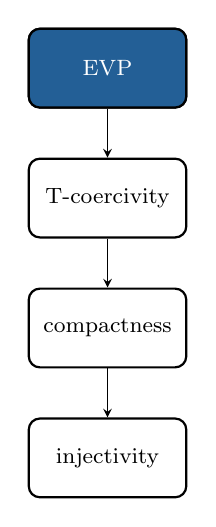
\begin{tikzpicture}[scale=1.1]
      \node (A) at (0,4.5) [draw,thick,minimum width=2cm,minimum height=1cm,rounded corners] {\footnotesize EVP};
      \node (B) at (0,3) [draw,thick,minimum width=2cm,minimum height=1cm,rounded corners] {\footnotesize T-coercivity};
      \node (C) at (0,1.5) [draw,thick,minimum width=2cm,minimum height=1cm,rounded corners] {\footnotesize compactness};
      \node (D) at (0,0) [draw,thick,minimum width=2cm,minimum height=1cm,rounded corners] {\footnotesize injectivity};
      \draw[-stealth] (A) -- (B);
      \draw[-stealth] (B) -- (C);
      \draw[-stealth] (C) -- (D);
      \node<1-> at (0,4.5) [draw,thick,minimum width=2cm,minimum height=1cm,rounded corners,fill=GOE] {\footnotesize \color{white} EVP};
    \end{tikzpicture}
  \end{minipage}
\end{frame}



\begin{frame}{Continuous Analysis: T-coercivity}
  \begin{minipage}{0.83\textwidth}
    \begin{itemize}
      \item<1->[\nicearrow{GOE}{-0.07cm}] $\exists$ eigenpairs $(\lami,\ei)_{i \in \mathbb{N}}$ of $e(\cdot,\cdot)$ s.t. $(\ei)_{i \in \mathbb{N}}$ forms an orthonormal basis of $X$
      \item<2->[\nicearrow{GOE}{-0.07cm}] set $i_{\ast} := \min \{ i \in \mathbb{N} : \lami < k^2 \}$ and define 
      \begin{equation*}
        W := \text{span}_{0 \le i \le i_{\ast}} \{ \ei \}, \qquad T := \Id_{X} - 2P_{W}
      \end{equation*}
      \item<3->[\nicearrow{GOE}{-0.07cm}] $T$ bijective \& acts on eigenfcts.~as $T \ei = \begin{cases}
        - \ei &\text{ if } \lami < k^2; \\
        + \ei &\text{ if } \lami > k^2.
      \end{cases}$
      \item<4->[\nicearrow{GOE}{-0.07cm}] We have that 
      \begin{align*}
        e(&Tu,u) - k^2(Tu,u)_{L^2} \\
        &= \sum_{i \le i_{\ast}} C_{\lambda} (k^2 - \lami)(\ui)^2 + \sum_{i > i_{\ast}} C_{\lambda} (\lami - k^2)(\ui)^2 \ge \gamma \Vert u \Vert^2_{X}
      \end{align*}
    \end{itemize}
  \end{minipage}
  \hfill
  \begin{minipage}{0.12\textwidth}
    \centering
    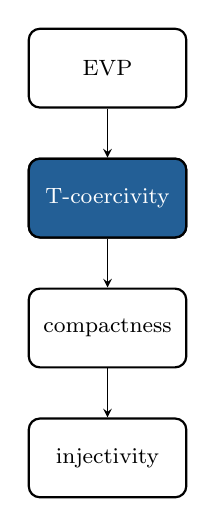
\begin{tikzpicture}[scale=1.1]
      \node (A) at (0,4.5) [draw,thick,minimum width=2cm,minimum height=1cm,rounded corners] {\footnotesize EVP};
      \node (B) at (0,3) [draw,thick,minimum width=2cm,minimum height=1cm,rounded corners] {\footnotesize T-coercivity};
      \node (C) at (0,1.5) [draw,thick,minimum width=2cm,minimum height=1cm,rounded corners] {\footnotesize compactness};
      \node (D) at (0,0) [draw,thick,minimum width=2cm,minimum height=1cm,rounded corners] {\footnotesize injectivity};
      \draw[-stealth] (A) -- (B);
      \draw[-stealth] (B) -- (C);
      \draw[-stealth] (C) -- (D);
      \node<1-> at (0,3) [draw,thick,minimum width=2cm,minimum height=1cm,rounded corners,fill=GOE] {\footnotesize \color{white} T-coercivity};
    \end{tikzpicture}
  \end{minipage}
\end{frame}


\begin{frame}{Continuous Analysis: compactness}
  \begin{minipage}{0.83\textwidth}
    Estimate each boundary term, e.g. for \emph{sound hard} BCs ($\beta = 0$)
    \begin{align*}
      \Vert K u \Vert_{X'} &= \sup_{v \in X \setminus \{ 0 \}} \frac{\vert \spl Ku,v \spr_{X',X} \vert}{\Vert v \Vert_{H^2(\Omega)}} \\
      &\le \sup_{v \in X \setminus \{ 0 \}} \frac{\vert \alpha \vert \Vert \gamma_0 \Delta u \Vert_{L^2(\partial \Omega)} \Vert \gamma_0 \nabla v \cdot \nv \Vert_{L^2(\partial \Omega)} \vert}{\Vert v \Vert_{H^2(\Omega)}} \\
      &\le C \vert \alpha \vert \Vert \gamma_0 \Delta u \Vert_{L^2(\partial \Omega)}
    \end{align*}
    \begin{itemize}
      \item<2->[\nicearrow{GOE}{-0.07cm}] last step uses continuity of normal trace operator
      \item<3->[\nicearrow{GOE}{-0.07cm}] Thus: $\forall (u_n)_{n \in \mathbb{N}} \subset H^2$ s.t. $u_n \overset{H^2}{\rightharpoonup} u$ $\Rightarrow$ $Ku_n \to Ku$, so $K$ is compact
      \item<4->[\nicearrow{GOE}{-0.07cm}] use similar arguments for $\beta > 0$ \& the \emph{impedance} case
    \end{itemize}
  \end{minipage}
  \hfill
  \begin{minipage}{0.12\textwidth}
    \centering
    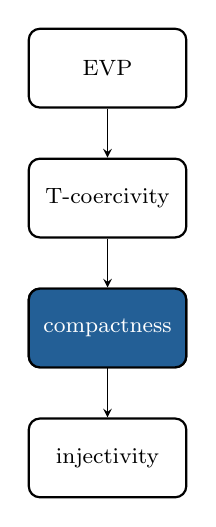
\begin{tikzpicture}[scale=1.1]
      \node (A) at (0,4.5) [draw,thick,minimum width=2cm,minimum height=1cm,rounded corners] {\footnotesize EVP};
      \node (B) at (0,3) [draw,thick,minimum width=2cm,minimum height=1cm,rounded corners] {\footnotesize T-coercivity};
      \node (C) at (0,1.5) [draw,thick,minimum width=2cm,minimum height=1cm,rounded corners] {\footnotesize compactness};
      \node (D) at (0,0) [draw,thick,minimum width=2cm,minimum height=1cm,rounded corners] {\footnotesize injectivity};
      \draw[-stealth] (A) -- (B);
      \draw[-stealth] (B) -- (C);
      \draw[-stealth] (C) -- (D);
      \node<1-> at (0,1.5) [draw,thick,minimum width=2cm,minimum height=1cm,rounded corners,fill=GOE] {\footnotesize \color{white} compactness};
    \end{tikzpicture}
  \end{minipage}
\end{frame}

\begin{frame}{Continuous Analysis: injectivity}
  \begin{minipage}{0.83\textwidth}
    \begin{itemize}
      \item<1->[\nicearrow{GOE}{-0.07cm}] need to assume that $k^2 \not \in \{ \lami \}_{i \in \mathbb{N}}$
      \item<2->[\nicearrow{GOE}{-0.07cm}] for \emph{impedance} case: take $v \in \ker a(\cdot,\cdot)$, then 
      \begin{equation*}
        0 = \vert - \Im a(v,v) \vert \ge \left \vert \frac{\alpha \zeta}{2} \Vert \Delta v \Vert^2_{L^2(\partial \Omega)} + \frac{\theta}{2 \zeta} \Vert v \Vert^2_{L^2(\partial \Omega)} \right \vert
      \end{equation*}
      \item<3->[\nicearrow{GOE}{-0.07cm}] $\gamma_0 v = 0$ and $\gamma_0 \Delta v = 0$ on $\partial \Omega$, use unique continuation principle to conclude that $v = 0$ in $\Omega$
    \end{itemize}
    \begin{block}{We have shown:}<4->
      $\mathcal{A}$ is (weakly) T-coercive and injective $\Rightarrow$ there $\exists ! u \in X$ s.t. $a(u,v) = (f,v)_{L^2(\Omega)}$ for all $v \in X$
    \end{block}
  \end{minipage}
  \hfill
  \begin{minipage}{0.12\textwidth}
    \centering
    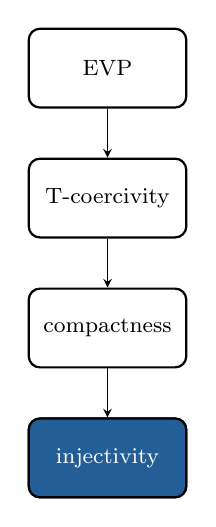
\begin{tikzpicture}[scale=1.1]
      \node (A) at (0,4.5) [draw,thick,minimum width=2cm,minimum height=1cm,rounded corners] {\footnotesize EVP};
      \node (B) at (0,3) [draw,thick,minimum width=2cm,minimum height=1cm,rounded corners] {\footnotesize T-coercivity};
      \node (C) at (0,1.5) [draw,thick,minimum width=2cm,minimum height=1cm,rounded corners] {\footnotesize compactness};
      \node (D) at (0,0) [draw,thick,minimum width=2cm,minimum height=1cm,rounded corners] {\footnotesize injectivity};
      \draw[-stealth] (A) -- (B);
      \draw[-stealth] (B) -- (C);
      \draw[-stealth] (C) -- (D);
      \node<1-> at (0,0) [draw,thick,minimum width=2cm,minimum height=1cm,rounded corners,fill=GOE] {\footnotesize \color{white} injectivity};
    \end{tikzpicture}
  \end{minipage}
\end{frame}

\section{Discrete problem}
\mysectionpage

\begin{frame}{Discretization}
  \begin{minipage}{0.7\textwidth}
    Let $\{ \mathcal{T}_h \}_{h}$ be a family of shape regular, quasi-uniform, simplicial triangulations. We choose an $H^2$-conforming finite element space, $p > 4$: 
    \begin{equation*}
      X_h := \{ v \in H^2(\Omega) : v \vert_{T} \in \mathcal{P}^p(T) \quad \forall T \in \mathcal{T}_h \} 
    \end{equation*}
    \begin{itemize}
      \item[\nicearrow{GOE}{-0.07cm}] imposing essential BCs for $\mathcal{C}^1$-conf.~FEM challenging\footnotemark; 
      \item[\nicearrow{GOE}{-0.07cm}] use Nitsche's method to impose BCs (for \emph{sound soft} \& \emph{sound hard}, not necessary for \emph{impedance})
    \end{itemize}
  \end{minipage}
  \hfill 
  \begin{minipage}{0.29\textwidth}
    \begin{center}
      \begin{tikzpicture}[scale=1.75]
        \node at (0.5,2.2) {\includegraphics[width=3.5cm,keepaspectratio]{ChristmasMesh/drawmesh.pdf}};
        \node[circle,fill=black,inner sep=0pt,minimum size=5pt] (A) at (0,0) {}; 
        \node[circle,fill=black,inner sep=0pt,minimum size=5pt]  (B) at (0,1) {};
        \node[circle,fill=black,inner sep=0pt,minimum size=5pt]  (C) at (1,0) {}; 
        \draw (A) -- (B) -- (C) -- (A);
        \foreach \nd in {A,B,C}{
          \draw (\nd) circle[radius=0.1];
          \draw (\nd) circle[radius=0.15];
        }
        \node at (0,0.5) {$\leftarrow$};
        \node at (0.5,0) {\rotatebox{90}{$\leftarrow$}};
        \node at (0.5,0) {\rotatebox{90}{$\leftarrow$}};
        \node at (0.5,0.5) {\rotatebox{225}{$\leftarrow$}};
        \node[align=center] at (0.5,-0.5) {\footnotesize Argyris-element, \\ \footnotesize $p \ge 5$};
      \end{tikzpicture}
    \end{center}
  \end{minipage}
  \footnotetext{\tiny R.C. Kirby, L. Mitchell, \emph{Code generation for generally mapped finite elements}. ACM TOMS, 2019.}
\end{frame}

\begin{frame}{Discrete problem}
  Find $u_h \in X_h$ s.t. $a_h(u_h,v_h) = (f,v_h)_{L^2(\Omega)}$ for all $v_h \in X_h$, where 
  \begin{equation*}
    a_h(u_h,v_h) := a(u_h,v_h) + \epsilon \left( \mathcal{N}_h(u_h,v_h) \right)
  \end{equation*}
  \begin{itemize}
    \item[\nicearrow{GOE}{-0.07cm}] $\epsilon = 0$ for \emph{impedance} BCs, $\epsilon = 1$ for \emph{sound soft} BCs
    \item[\nicearrow{GOE}{-0.07cm}] discrete analysis follows similar steps as the continuous case:
    \begin{enumerate}
      \item analyse the discrete EVP (with potential Nitsche terms);
      \item construct T$_h$ and show uniform T$_h$-coercivity;
    \end{enumerate}
    \item[\nicearrow{GOE}{-0.07cm}] for \emph{impedance} BCs ($\epsilon = 0$), we can neglect the compact term 
    \item[\nicearrow{GOE}{-0.07cm}] \emph{sound hard} BCs can be analyzed with similar arguments
  \end{itemize}
\end{frame}

\begin{frame}{Nitsche terms}
  \begin{minipage}{0.75\textwidth}
    \begin{align*}
      \mathcal{N}_h(u_h,v_h) := &\alpha (\nabla(\Delta u_h) \cdot \bm{\nu}, v_h)_{L^2(\partial \Omega)} - (\nabla u_h \cdot \bm{\nu}, v_h)_{L^2(\partial \Omega)} \\
      + &\beta (\nabla(\bm{n}^T (\mathcal{H}u_h) \bm{n}) \cdot \bm{\nu}, v_h)_{L^2(\partial \Omega)} \\[0.2cm]
      + &\alpha (u_h,\nabla(\Delta v_h) \cdot \bm{\nu})_{L^2(\partial \Omega)} - (u_h,\nabla v_h \cdot \bm{\nu})_{L^2(\partial \Omega)} \\
      + &\beta (u_h, \nabla (\bm{n}^T (\mathcal{H}v_h) \bm{n}) \cdot \bm{\nu})_{L^2(\partial \Omega)} \\[0.2cm]
      + &\alpha \frac{\eta_1}{h^3} (u_h,v_h)_{L^2(\partial \Omega)} + \frac{\eta_2}{h} (u_h,v_h)_{L^2(\partial \Omega)} \\
      + &\beta \frac{\eta_3}{h^3} (u_h,v_h)_{L^2(\partial \Omega)}
    \end{align*}
  \end{minipage}
  \hfill
  \begin{minipage}{0.24\textwidth}
  \end{minipage}
  \begin{center}
    \begin{tikzpicture}[overlay,yshift=-0.3cm]
      \node<2-> at (4,4.35) {\color{gray!75} \scalebox{3.35}{\}} };
      \node<3-> at (4,2.75) {\color{gray!75} \scalebox{3.35}{\}} };
      \node<4-> at (4,1.25) {\color{gray!75} \scalebox{3.35}{\}} };
      \node<2->[align=center] at (6,4.35) {\footnotesize \color{gray!75} natural boundary \\ \footnotesize \color{gray!75} terms};
      \node<3->[align=center] at (6,2.75) {\footnotesize \color{gray!75} symmetry \\ \footnotesize \color{gray!75} terms};
      \node<4->[align=center] at (6,1.25) {\footnotesize \color{gray!75} penalty \\ \footnotesize \color{gray!75} terms};
    \end{tikzpicture}
  \end{center}
  \uncover<5->{
  \vspace*{-0.2cm}
  \begin{align*}
    \nicearrow{GOE}{-0.07cm} \quad \vert \mathcal{N}_h(u_h,u_h) \vert \gtrsim &- \frac{\alpha \zeta_1}{h^3} \Vert \Delta u_h \Vert^2_{L^2(\Omega)} - \frac{\zeta_2}{h} \Vert \nabla u_h \Vert^2_{L^2(\Omega)} -  \frac{\beta \zeta_3}{h^3} \vert u \vert^2_{H^2(\Omega)} \\
    &+ \left( \frac{\alpha \eta_1}{h^3} - \frac{\alpha}{\zeta_1} + \frac{\eta_2}{h} - \frac{1}{\zeta_2} + \frac{\beta \eta_3}{h^3} - \frac{\beta}{\zeta_3} \right) \Vert u \Vert^2_{L^2(\partial \Omega)} 
  \end{align*}}
\end{frame}

\begin{frame}{Discrete EVP}
  Find $u_h \in \tilde{X}_h \subseteq X_h$, $\lambda \in \mathbb{C}$, s.t. for all $v_h \in \tilde{X}_h$
  \begin{equation*}
    e_h(u_h,v_h) := e(u_h,v_h) + \epsilon \mathcal{N}_h(u_h,v_h) = \lambda (u_h,v_h)_{L^2(\Omega)} 
  \end{equation*}
  \begin{itemize}
    \item<2->[\nicearrow{GOE}{-0.07cm}]  $\tilde{X}_h = X_h$ if $\epsilon = 1$, $\tilde{X}_h = X_h \cap \{ u_h = 0 \text{ on } \partial \Omega \} \cap \{ \Delta u_h = 0 \text{ on } \partial \Omega \}$ if $\epsilon = 0$
    \item<3->[\nicearrow{GOE}{-0.07cm}] Discrete norm: $\Vert u_h \Vert_{\epsilon}^2 := \vert u_h \vert^2_{H^2(\Omega)} + \vert u_h \vert^2_{H^1(\Omega)} + \epsilon \Vert u \Vert^2_{L^2(\partial \Omega)}$
  \end{itemize}
  \begin{lemma}<4->
    For $\eta_i$, $i = 1,2,3$, large enough, the bilinear form $e_h(\cdot,\cdot)$ is uniformly coercive on $\tilde{X}_h$ w.r.t. $\Vert \cdot \Vert_{\epsilon}$. 
  \end{lemma}
  \begin{proof}<5->
    Use the estimate for $\mathcal{N}_h(\cdot,\cdot)$ from the previous slide \& choose $\zeta_i$ small enough, $\eta_i$ large enough, $i = 1,2,3$.
  \end{proof}
\end{frame}


\begin{frame}{Discrete T$_h$-coercivity}
  \begin{itemize}
    \item[\nicearrow{GOE}{-0.07cm}] define $T_h \in L(X_h)$ s.t $T \ei_h = \begin{cases}
      - \ei_h &\text{ if } i \le i_{\ast}; \\
      + \ei_h &\text{ if } i > i_{\ast}.
    \end{cases}$
    \item<2->[\nicearrow{GOE}{-0.07cm}] as in the continuous case, we have that 
    \begin{align*}
      &e_h(T_h u_h,u_h) - k^2(T_h u_h,u_h) \\
      = &\sum_{0 \le i \le i_{\ast}} C_{\lambda_h} (k^2 - \lami_h) (\ui_h)^2 + \sum_{i > i_{\ast}} C_{\lambda_h} (\lami_h - k^2) (\ui_h)^2 \ge \gamma \Vert u_h \Vert^2_{\epsilon},
    \end{align*}
    if $h$ is \alert{small enough} s.t. $\lambda_h^{(i_{\ast})} < k^2$.
    \item<3->[\nicearrow{GOE}{-0.07cm}] (there $\exists h_0$ s.t. $\forall h \le h_0$) $a_h(\cdot,\cdot)$ is uniformly T$_h$-coercive
    \item<4->[\nicearrow{GOE}{-0.07cm}] the discrete problem has a unique solution for $h$ small enough
  \end{itemize}
\end{frame}

\begin{frame}{Best approximation}
  \begin{itemize}
    \item[\nicearrow{GOE}{-0.07cm}] $a_h(\cdot,\cdot)$ is \alert{continuous} wrt (stronger) $\Vert \cdot \Vert_{h,\epsilon}$-norm: 
    \begin{equation*}
      \Vert u_h \Vert_{h,\epsilon}^2 := \Vert u_h \Vert^2_{\epsilon} + \epsilon \left( h^3 \Vert \nabla(\Delta u_h) \Vert^2_{L^2(\partial \Omega)} + h^3 \Vert \nabla(\bm{n}^T \mathcal{H} u_h \bm{n}) \Vert^2_{L^2(\Omega)} + h \Vert \nabla u_h \Vert_{L^2(\partial \Omega)} \right)
    \end{equation*}
    \item<2->[\nicearrow{GOE}{-0.07cm}] $a_h$ is \alert{consistent}, i.e. $a_h(u-u_n,v_h) = 0$ for all $v_h \in X_h$
    \item<3->[\nicearrow{GOE}{-0.07cm}] with classical arguments, we can show that 
    \begin{equation*}
      \Vert u - u_h \Vert_{h,\epsilon} \le C \inf_{v_h \in X_h} \Vert u - v_h \Vert_{h,\epsilon}.
    \end{equation*}
  \end{itemize}
\end{frame}


\section{Numerical examples}
\mysectionpage

\begin{frame}{Manufactured Solution}
  \begin{minipage}{0.49\textwidth}
    \begin{itemize}
      \item<1->[\nicearrow{GOE}{-0.07cm}] plane wave solution $u(\bm{x}) = e^{i \bm{d} \cdot \bm{x}}$, choose $\bm{d} \in \mathbb{C}^d$ s.t. $u$ solves the nematic Helmholtz--Korteweg eqs. 
      \item<2->[\nicearrow{GOE}{-0.07cm}] for $u \in H^5(\Omega)$, we can construct $I_h : u \to X_h$ s.t. 
      \begin{equation*}
        \Vert u - I_h u \Vert_{H^2(\Omega)} \le h^3 \Vert u \Vert_{H^5(\Omega)} 
      \end{equation*} 
      \item<3->[\nicearrow{GOE}{-0.07cm}] dashed: $k = 20$, solid: $k = 30$
    \end{itemize}
  \end{minipage}
  \hfill
  \begin{minipage}{0.49\textwidth}
    \uncover<3->{
    \begin{tikzpicture}[scale=1]
      \begin{axis}[ymode=log, 
                   grid style=dashed, 
                   xlabel={Ref.~ lvl.}, 
                   ylabel={$\lVert u-u_h \rVert_{H^2(\Omega)}$}, 
                   title={$\alpha=10^{-2}$}, 
                   legend pos=south west, 
                   legend cell align={left},
                   width=7cm,
                   cycle list name=unfmixed2
                  ]
        \addplot table [x=refs, y=H2, col sep=comma] {assets/convergence_30.0_0.01_0.0.csv};
        \addplot table [x=refs, y=H2, col sep=comma] {assets/convergence_30.0_0.01_0.005.csv};
        \addplot table [x=refs, y=H2, col sep=comma] {assets/convergence_20.0_0.01_0.0.csv};
        \addplot table [x=refs, y=H2, col sep=comma] {assets/convergence_20.0_0.01_0.005.csv};
        \addplot[gray,dashed,domain=1:4] {0.125*((1/16)^x)};
        \legend{$\beta=0$, $\beta=5\cdot 10^{-3}$}
      \end{axis}
    \end{tikzpicture}}
  \end{minipage}
\end{frame}

\begin{frame}{Gaussian pulse}
  \begin{overlayarea}{\textwidth}{\textheight}
  \nicearrow{GOE}{-0.07cm} rhs: symmetric Gaussian pulse in $(0,0)$, \emph{impedance} BCs, $k = 40$, $\alpha = 10^{-2}$
  \begin{center}
    \begin{tikzpicture}[scale=1.1]
      \node at (-4,0) {\includegraphics[width=0.23\textwidth,keepaspectratio]{figures/GPIM.png}};
      \node at (-1,0) {\includegraphics[width=0.23\textwidth,keepaspectratio]{figures/GPIM-X.png}};
      \node at (2,0) {\includegraphics[width=0.23\textwidth,keepaspectratio]{figures/GPIM-XY.png}};
      \node at (5,0) {\includegraphics[width=0.23\textwidth,keepaspectratio]{figures/GPIM-Y.png}};
      \node at (-4,-1.75) {\footnotesize $\beta = 0$};
      \node at (-1,-1.75) {\footnotesize $\beta = 5\cdot 10^{-3}$};
      \node at (2,-1.75) {\footnotesize $\beta = 5\cdot 10^{-3}$};
      \node at (5,-1.75) {\footnotesize $\beta = 5\cdot 10^{-3}$};
      \begin{scope}[yshift=0.2cm]
        \draw<2->[stealth-stealth,line width=1.65pt,color=white] (-1.75,-1) -- (-0.25,-1);
        \draw<2->[stealth-stealth,line width=1.65pt,color=white] (-1.75,-1.25) -- (-0.25,-1.25);
        \draw<2->[stealth-stealth,line width=1.65pt,color=white] (-1.75,-1.5) -- (-0.25,-1.5);
      \end{scope}
      \draw<2->[stealth-stealth,line width=1.65pt,color=white] (4.5,-0.95) -- (4.5,0.55);
      \draw<2->[stealth-stealth,line width=1.65pt,color=white] (4.25,-0.95) -- (4.25,0.55);
      \draw<2->[stealth-stealth,line width=1.65pt,color=white] (4.0,-0.95) -- (4.0,0.55);
      \begin{scope}[rotate=45,xshift=-0.65cm,yshift=0.3cm]
        \draw<2->[stealth-stealth,line width=1.65pt,color=white] (1.25,-1) -- (2.75,-1);
        \draw<2->[stealth-stealth,line width=1.65pt,color=white] (1.25,-1.25) -- (2.75,-1.25);
        \draw<2->[stealth-stealth,line width=1.65pt,color=white] (1.25,-1.5) -- (2.75,-1.5);
      \end{scope}
    \end{tikzpicture}
  \end{center}
\end{overlayarea}
\end{frame}

\begin{frame}{Mullen-L\"uthi-Stephen experiment\footnotemark}
  \begin{center}
    \begin{tikzpicture}
      \node at(0,0) {\includegraphics[width=0.4\textwidth,keepaspectratio]{figures/MLSXYX.png}};
      \node at(6,0) {\includegraphics[width=0.4\textwidth,keepaspectratio]{figures/MLSYXY.png}};
      \begin{scope}[yshift=-1cm]
        \draw<1->[-stealth,line width=1.65pt,color=white] (5,-1) -- (7,-1);
        \draw<1->[-stealth,line width=1.65pt,color=white] (5,-1.25) -- (7,-1.25);
        \draw<1->[-stealth,line width=1.65pt,color=white] (5,-1.5) -- (7,-1.5);
        \draw<1->[-stealth,line width=1.65pt,color=white] (4.5,-1.65) -- (4.5,-0.85);
        \draw<1->[-stealth,line width=1.65pt,color=white] (4.25,-1.65) -- (4.25,-0.85);
        \draw<1->[-stealth,line width=1.65pt,color=white] (4.0,-1.65) -- (4.0,-0.85);
        \draw<1->[-stealth,line width=1.65pt,color=white] (7.5,-1.65) -- (7.5,-0.85);
        \draw<1->[-stealth,line width=1.65pt,color=white] (7.75,-1.65) -- (7.75,-0.85);
        \draw<1->[-stealth,line width=1.65pt,color=white] (8.0,-1.65) -- (8.0,-0.85);
      \end{scope}
      \begin{scope}[yshift=-1cm]
        \draw<1->[-stealth,line width=1.65pt,color=white] (-2,-1) -- (-1,-1);
        \draw<1->[-stealth,line width=1.65pt,color=white] (-2,-1.25) -- (-1,-1.25);
        \draw<1->[-stealth,line width=1.65pt,color=white] (-2,-1.5) -- (-1,-1.5);
        \draw<1->[-stealth,line width=1.65pt,color=white] (1,-1) -- (2,-1);
        \draw<1->[-stealth,line width=1.65pt,color=white] (1,-1.25) -- (2,-1.25);
        \draw<1->[-stealth,line width=1.65pt,color=white] (1,-1.5) -- (2,-1.5);
        \draw<1->[-stealth,line width=1.65pt,color=white] (0,-1.65) -- (0,-0.85);
        \draw<1->[-stealth,line width=1.65pt,color=white] (-0.5,-1.65) -- (-0.5,-0.85);
        \draw<1->[-stealth,line width=1.65pt,color=white] (0.5,-1.65) -- (0.5,-0.85);
        \draw<1->[-stealth,line width=1.65pt,color=white] (-0.25,-1.65) -- (-0.25,-0.85);
        \draw<1->[-stealth,line width=1.65pt,color=white] (0.25,-1.65) -- (0.25,-0.85);
      \end{scope}
    \end{tikzpicture}
  \end{center}
  \footnotetext[6]{\tiny M.E. Mullen, B. L\"uthi, M.J. Stephen, \emph{Sound velocity in a nematic liquid crystal}. Physics review letters, 1972.}
\end{frame}


\begin{frame}{Conclusion}
  \begin{overlayarea}{\textwidth}{\textheight}
  \begin{itemize}
    \item<1->[\nicearrow{GOE}{-0.07cm}] we showed well-posedness of the (continuous) nematic Helmholtz--Korteweg equations
    \begin{itemize}
      \item[\MVRightArrow] (weak) T-coercivity argument where $T$ flips the sign of 'problematic' eigenfcts.
      \item[\MVRightArrow] analysis appplies to \emph{sound soft}, \emph{sound hard} \& \emph{impedance} BCs  
    \end{itemize}
    \item<2->[\nicearrow{GOE}{-0.07cm}] we analysed the discretization with $H^2$-conforming FEM 
    \begin{itemize}
      \item[\MVRightArrow] imposition of essential BCs through Nitsche's method
      \item[\MVRightArrow] transfer T-coercivity arguments to the discrete level  
    \end{itemize}
    \item<3->[\nicearrow{GOE}{-0.07cm}] numerical experiments to study the effect of the nematic field on the propagation of acoustic waves
  \end{itemize}
  \begin{center}
    
\begin{tikzpicture}
      \node<4-> at (0,0) {\LARGE \textbf{Thank you for your attention!}};
    \end{tikzpicture}
  \end{center}
\end{overlayarea}
\end{frame}


\end{document}